\begin{table}[!hbt]
	\centering
	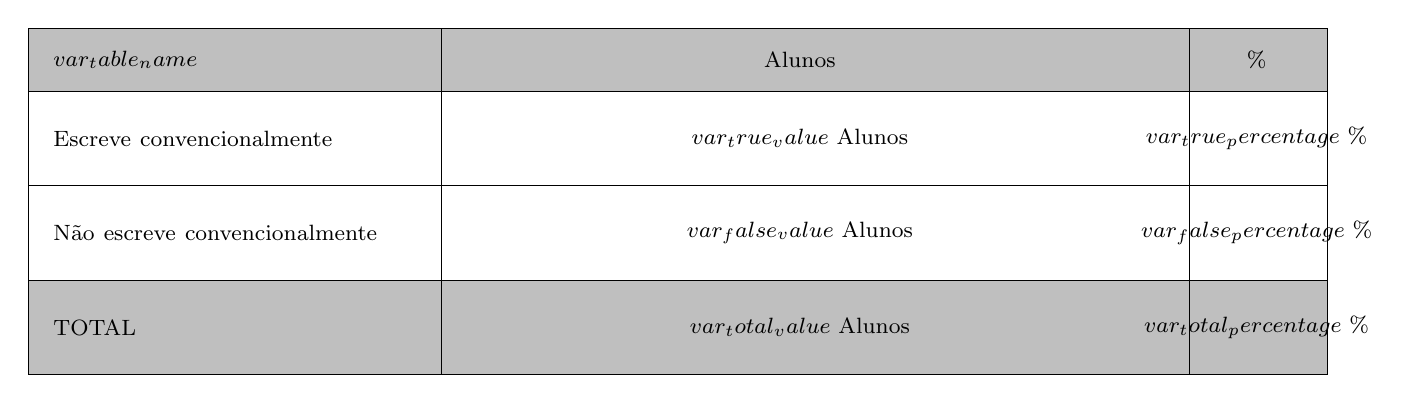
\begin{tikzpicture}
		\fill[lightgray] (-8.25,-1.1) rectangle (8.25,-0.3);
		\fill[lightgray] (-8.25,-3.5) rectangle (8.25,-4.7);
		\draw (-8.25,-0.3) rectangle (8.25,-4.7);
		\draw (-8.25,-1.1) -- (8.25,-1.1);
		\draw (-8.25,-2.3) -- (8.25,-2.3);
		\draw (-8.25,-3.5) -- (8.25,-3.5);

		\draw (-3,-0.3) -- (-3,-4.7);
		\draw (6.5,-0.3) -- (6.5,-4.7);

        \node[text width=6cm] at (-4.93,-0.7) {\fontsize{8}{0}\selectfont $var_table_name$};
		\node[text width=6cm] at (-4.93,-1.7) {\fontsize{8}{0}\selectfont Escreve convencionalmente};
		\node[text width=6cm] at (-4.93,-2.9) {\fontsize{8}{0}\selectfont Não escreve convencionalmente};
		\node[text width=6cm] at (-4.93,-4.1) {\fontsize{8}{0}\selectfont TOTAL};

		\node at (1.55,-0.7) {\fontsize{8}{0}\selectfont Alunos};
		\node at (7.35,-0.7) {\fontsize{8}{0}\selectfont \%};

		\node at (1.55,-1.7) {\fontsize{8}{0}\selectfont $var_true_value$ Alunos};
		\node at (7.35,-1.7) {\fontsize{8}{0}\selectfont $var_true_percentage$ \%};

		\node at (1.55,-2.9) {\fontsize{8}{0}\selectfont $var_false_value$ Alunos};
		\node at (7.35,-2.9) {\fontsize{8}{0}\selectfont $var_false_percentage$ \%};

		\node at (1.55,-4.1) {\fontsize{8}{0}\selectfont $var_total_value$ Alunos};
		\node at (7.35,-4.1) {\fontsize{8}{0}\selectfont $var_total_percentage$ \%};
	\end{tikzpicture}
\end{table}